\documentclass[]{article}
\usepackage{amsmath}
\usepackage{graphicx}
\usepackage{tikz}
\usetikzlibrary{positioning,shapes,arrows}



\begin{document}
\title{Fundamentals of Artificial Intelligence:\\Constraint Processing Assignment}
\author{Shiva HosseiniTehrani}
\maketitle

Constraint Programming is widely use in operations research. It is finding a feasible solution rather than optimization and focuses on the constraints and variables domain rather than the objective function.
\\
constraint programming exploit constraints during tree search\\
1. Use propagation algorithms for constraints\\
2. Employ branching algorithm\\
3. Execute exploration algorithm\\


\section{Summation problem}
Given a set of even number representing with squares and given a set of odd number representing with circles in the range of [1,6]. The problem refers to assigning numbers to the circles and squares such that:\\
1. The summation of most right digit of the first number which is even and the most right digit of the second number which is an odd number should be odd.
2. The summation of the middle digit of the first number which is even and the middle digit of the second number which is odd and the possible carry should be an even number.
3. The summation of the most left digit of the first number which is odd and the most left digit of the second number which is even and the possible carry should be odd.

We have specified each digit with a variable, as it has shown in figure \ref{fig:fig0}.
\\
\begin{figure}[h]
\centering
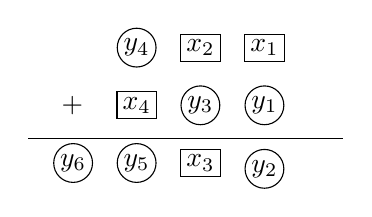
\begin{tikzpicture}[
node distance=0.3cm and 0.3 cm,
  cnode/.style={draw,circle,inner sep=1pt},
  rnode/.style={draw,rectangle,inner sep=2pt}
]
\node[rnode] (P) {$x_1$};
\node[rnode,left=of P] (T) {$x_2$};
\node[cnode,left=of T](W) {$y_4$};
\node[cnode,below=of P] (A) {$y_1$};
\node[cnode,below=of T] (B) {$y_3$};
\node[rnode,below=of W] (C) {$x_4$};
\node[cnode,below=of A] (Q) {$y_2$};
\node[rnode,below=of B] (D) {$x_3$};
\node[cnode,below=of C] (K) {$y_5$};
\node[cnode,left=of  K] (R) {$y_6$};
\node [left=of C] {+};
\draw (-3,-1.15) -- (1,-1.15);
\end{tikzpicture}
\label{fig:fig0}
\end{figure}
 
Summation problem can be modeled as a constraint satisfaction problem (CSP), 
with the following properties:
\textbf{Set of variables:}\\
Even numbers : $x_1, x_2,x_3, x_4$\\
Odd numbers : $y_1, y_2, y_3, y_4, y_5,y_6$\\
Carries : $z_1, z_2$\\
\textbf{The domain of the variables:}\\
For {$x_1 - x_4$} the domain is: [2, 4, 6]\\
For {$y_1 - y_6$} the domain is: [1, 3, 5]\\
For {$z_1, z_2$} the domain is: [1]\\
\textbf{A set of constraints:}
\begin{align*}
x_1 + y_1 = y_2 + 10 * z_1 \\
x_2 + y_3 = x_3 + 10 * z_2 \\
x_4 + y_4 = y_5 + 10 * y_6 \\
\end{align*}
A solution is an assignment of a value in domain to each variable such that every constraint satisfied.

\section{Stacking squares}
In stacking squares the problem is locating a 5X5, 4X4, 3X3, 2X2 in a 9X7 rectangle in a way that non of the squares overlaps, squares can not be rotated and only the integer coordinates should be used in locating the corners of the squares.
\subsection*{part(1)}
Summation problem can be modeled as a constraint satisfaction problem (CSP), 
with the following properties:\\

\begin{itemize}

\item{Set of variables:}

\begin{align*}
&S2_c, S2_r, S3_c, S3_r, S2_r, S4c, S4_r, S5_c, S5_r\\
&col(i) 0\leq i \leq 62\\ 
&row(i) 0\leq i \leq 62\\
&Z(i)   0\leq i \leq 62\\
\end{align*}
$S2_c$ and $S2_r$ are indicating the column and row of top left corner of $2X2$ square, $S3_c$ and $S3_r$ are indicating the column and row of top left corner of $3X3$ square and so on. 
$col(i)$ and $row(i)$ represent the column and row of the element $i$ respectively.
$Z(i)$ denotes each cell of the rectangle that can be an element of $2X2$ or $3X3$ or $4X4$ or $5X5$.
\item{The domain of the variables:}

\begin{align*}
&S2_c \in [0, 7], S2_r \in [0, 5]\\
&S3_c \in [0, 6], S3_r \in [0, 4]\\
&S2_c \in [0, 5], S4_r \in [0, 3]\\
&S4_c \in [0, 4], S5_r \in [0, 2]\\
&col(i) \in [0, 8]\\
&row(i) \in [0, 6]\\
&Z(i) \in [1,5]\\
\end{align*}
\\
The first domain indicates that the top left corner of the $2X2$ square could be placed in column $[0, 7]$ and row $[0, 5]$, i.e (if it is placed in column 8 or row 6 the square will be located outside of the $9X7$ rectangle), the second, third and forth domain has the same view in different range for $3X3$, $4X4$ and $5X5$ respectively.
The fifth and sixth domain are indicating the range of column and row of each element in $9X7$ rectangle, which can be obtained by the following formula: \\
\begin{align*}  
col(i) = i \mod 9 \quad 0 \leq i \leq 62\\
row(i) = \lfloor \frac{i}{9}\rfloor  \quad 0 \leq i \leq 62 \\
\end{align*}
\\
\item{set of constraints:}

\begin{align*}
Z(i)= 2 \Leftrightarrow &col(i)-1 \leq S2_c \leq col(i) \land \\
&row(i)-1 \leq S2_c \leq row(i)\\
Z(i)= 3 \Leftrightarrow &col(i)-2 \leq S3_c \leq col(i) \land \\
&row(i)-2 \leq S3_c \leq row(i)\\
Z(i)= 4 \Leftrightarrow &col(i)-3 \leq S4_c \leq col(i) \land \\
&row(i)-3 \leq S4_c \leq row(i)\\
Z(i)= 5 \Leftrightarrow &col(i)-4 \leq S5_c \leq col(i) \land \\
&row(i)-4 \leq S5_c \leq row(i)\\
col(i) = i \mod 9 \quad  0 \leq i \leq 62\\
row(i) = i / 9    \quad  0 \leq i \leq 62 \\
\end{align*}
The first constraint indicates the fact that a variable $Z(i)$ (which can be 0 to 69) can be filled with $2X2$ square if and only if, the top left corner of those elements could be placed in $Z(i)= 2 \Leftrightarrow col(i)-1 \leq S2_c \leq col(i)$ and $row(i)-1 \leq S2_c \leq row(i)$. For instance in figure \ref{fig:rectangle}  $Z(20) = 2$ if and only if $S2C = [1,2]$ and  $S2R = [1,2]$ The rest of constraint has the same view in different range for $3X3$, $4X4$ and $5X5$ respectively.
\begin{figure}[h]
\centering
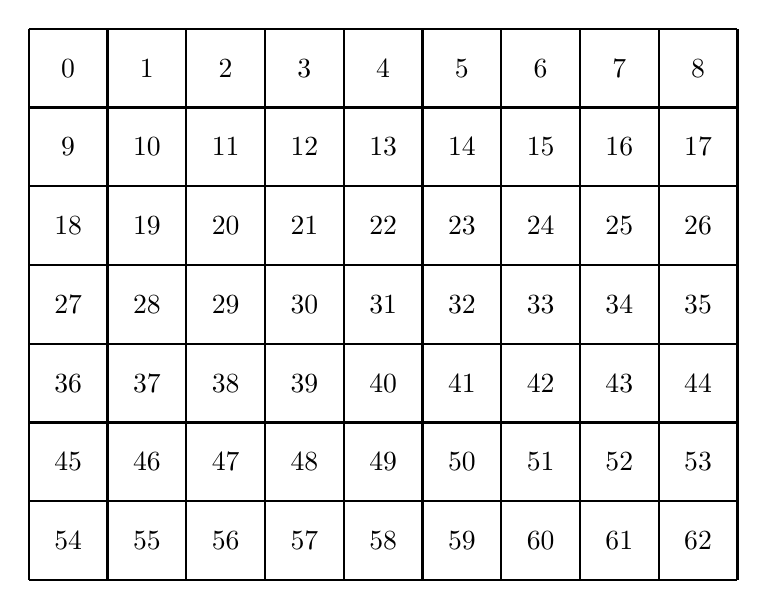
\begin{tikzpicture}[mysquare/.style = {draw=black, fill opacity = 0.5}]
\draw[step=1cm,black,thick] (0,0) grid (9,7);
%\fill[red!40!white,draw=black, mysquare] (2,5) rectangle (3,6)
\foreach \x in {0,...,8} 
    \foreach \y in {0,...,6} 
        \node at (\x + 0.5,\y + 0.5) {\pgfmathparse{int(9*(6-\y)  + \x)}\pgfmathresult};
\end{tikzpicture}
\caption{Board}
\label{fig:rectangle}
\end{figure}

\end{itemize}

\subsection*{part(2)}
\begin{figure}[h]
\centering
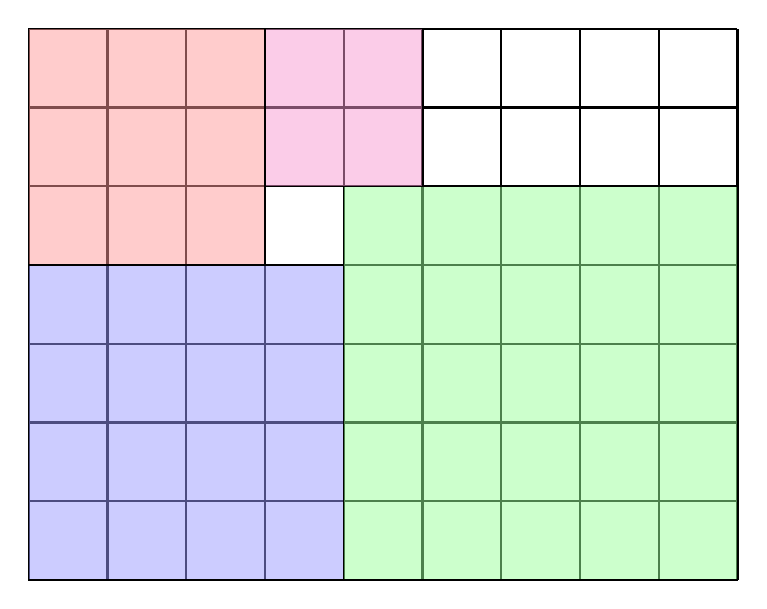
\begin{tikzpicture}[mysquare/.style = {draw=black, fill opacity = 0.5}]
\draw[step=1cm,black,thick] (0,0) grid (9,7);
\fill[blue!40!white,mysquare] (0,0) rectangle (4,4);
\fill[red!40!white,draw=black, mysquare] (0,4) rectangle (3,7);
\fill[magenta!40!white, mysquare] (3,5) rectangle (5,7);
\fill[green!40!white, mysquare] (4,0) rectangle (9,5);
\end{tikzpicture}
\caption{Caption}
\label{fig:rectangle}
\end{figure}

\section{Docked ships}


\begin{figure}[h]
\centering
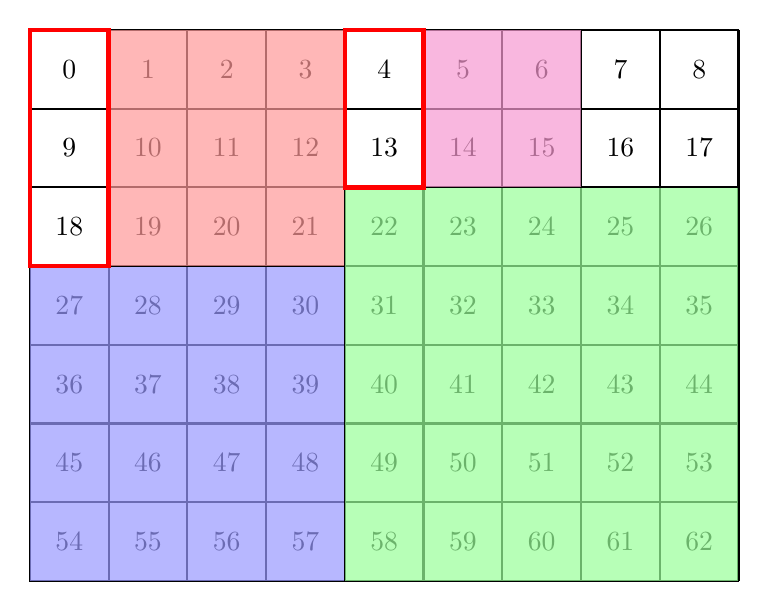
\begin{tikzpicture}[mysquare/.style = {draw=black, fill opacity = 0.7}]
\draw[step=1cm,black,thick] (0,0) grid (9,7);
\foreach \x in {0,...,8} 
    \foreach \y in {0,...,6} 
        \node at (\x + 0.5,\y + 0.5) {\pgfmathparse{int(9*(6-\y)  + \x)}\pgfmathresult};
\fill[blue!40!white,mysquare] (0,0) rectangle (4,4);
\fill[red!40!white,draw=black, mysquare] (1,4) rectangle (4,7);
\fill[magenta!40!white, mysquare] (5,5) rectangle (7,7);
\fill[green!40!white, mysquare] (4,0) rectangle (9,5);
\draw[red,ultra thick] (0,4) rectangle (1,7);
\draw[red,ultra thick] (4,5) rectangle (5,7);
\end{tikzpicture}
\caption{Placement of squares with vertical holes}
\label{fig:rectangleHole}
\end{figure}


\begin{figure}[h]
\centering
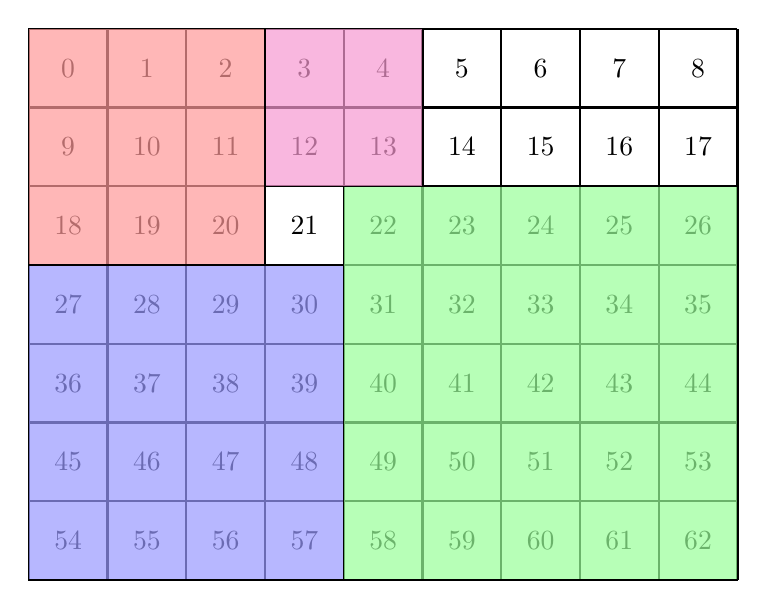
\begin{tikzpicture}[mysquare/.style = {draw=black, fill opacity = 0.7}]
\draw[step=1cm,black,thick] (0,0) grid (9,7);
\foreach \x in {0,...,8} 
    \foreach \y in {0,...,6} 
        \node at (\x + 0.5,\y + 0.5) {\pgfmathparse{int(9*(6-\y)  + \x)}\pgfmathresult};
\fill[blue!40!white,mysquare] (0,0) rectangle (4,4);
\fill[red!40!white,draw=black, mysquare] (0,4) rectangle (3,7);
\fill[magenta!40!white, mysquare] (3,5) rectangle (5,7);
\fill[green!40!white, mysquare] (4,0) rectangle (9,5);
\end{tikzpicture}
\caption{Placement of squares without holes}
\label{fig:rectangleNoHole}
\end{figure}

\end{document}